\chapter{Grundlagen}
\section{Historie}
Seit dem Beginn des Industriezeitalters um 1800, welches mit der Mechanisierung (Industrie 1.0) startete, befindet sich die Industrie in einem stetigen Wandel. Sie entwickelte sich um 1900 durch die Massenproduktion zur Industrie 2.0 und in den 1970er Jahren durch die Automatisierung zur Industrie 3.0. Die Einteilung der Industriezeitalter ist durch tiefgreifende Veränderungen im technologischen Fortschritt möglich, welche auch als industrielle Revolution bezeichnet werden. Aktuell befinden wir uns in der Phase der 4. industriellen Revolution.

\subsection{1. industrielle Revolution}
Die 1. industrielle Revolution fand mit der Erfindung der Dampfmaschine statt. Sie ermöglichte es Eisenbahnen und Dampfschiffe sowie verschiedene Maschinen im Kohleabbau oder in Textilfabriken anzutreiben und trug massiv zur Industrialisierung und der Entstehung der Industrie 1.0 bei. Nach und nach wurden immer mehr Produktionsanlagen errichtet und somit Arbeitsplätze in Infrastruktur, Textilfabriken, Häuserbau, Kohleabbau und anderen Bereichen geschaffen.

\subsection{2. industrielle Revolution}
Die Erforschung der Elektrizität im 19. Jahrhundert war der Auslöser der 2. industriellen Revolution. Nachdem ab 1830 die Gesetze der Elektrotechnik bekannt waren, fand die Elektrizität eine breite Anwendung in der Industrie und im Alltag. Im Jahr 1913 führte Henry Ford das Fließband in der Automobilbranche ein. Im Zuge dessen musste jeder Arbeiter nur noch einen Arbeitsschritt erledigen, welches einerseits die Produktion wesentlich beschleunigte und eine Massenproduktion ermöglichte und andererseits eine hohe Spezialisierung der einzelnen Arbeitskräfte für ihre bestimmte Aufgabe erforderte.

Außerdem wurde es durch die Luftfahrt möglich Produkte wie Autos, Kleidung und Lebensmittel über Kontinente hinweg immer schneller zu transportieren und zu handeln.

\subsection{3. industrielle Revolution}
Die 3. industrielle Revolution fand in den 1970er Jahren statt. Sie ist durch eine sukzessive (Teil-) Automatisierung der Prozesse und durch den Einzug der IT in die Industrie- und Verbraucherwelt geprägt. In den 1940er Jahren wurden die ersten Rechenmaschinen und programmierbare Steuerungen in Unternehmen eingesetzt. In den 1970er Jahren zog der Computer auch in den Privatbereich ein, wurde zunehmend beliebter und schaffte einen neuen Industriezweig. Der Fertigungsprozess in Fabriken wurde mehr und mehr von Maschinen übernommen.

Durch den zunehmenden Einsatz von IT in Unternehmen entstand immer mehr Kommunikation zwischen Menschen und Maschinenn. Diese Kommunikation und die anfallenden Daten wurden jedoch nur unternehmensintern verarbeitet. Es gab nur wenige Schnittstellen nach außen.

\begin{figure}[h]
  \centering
  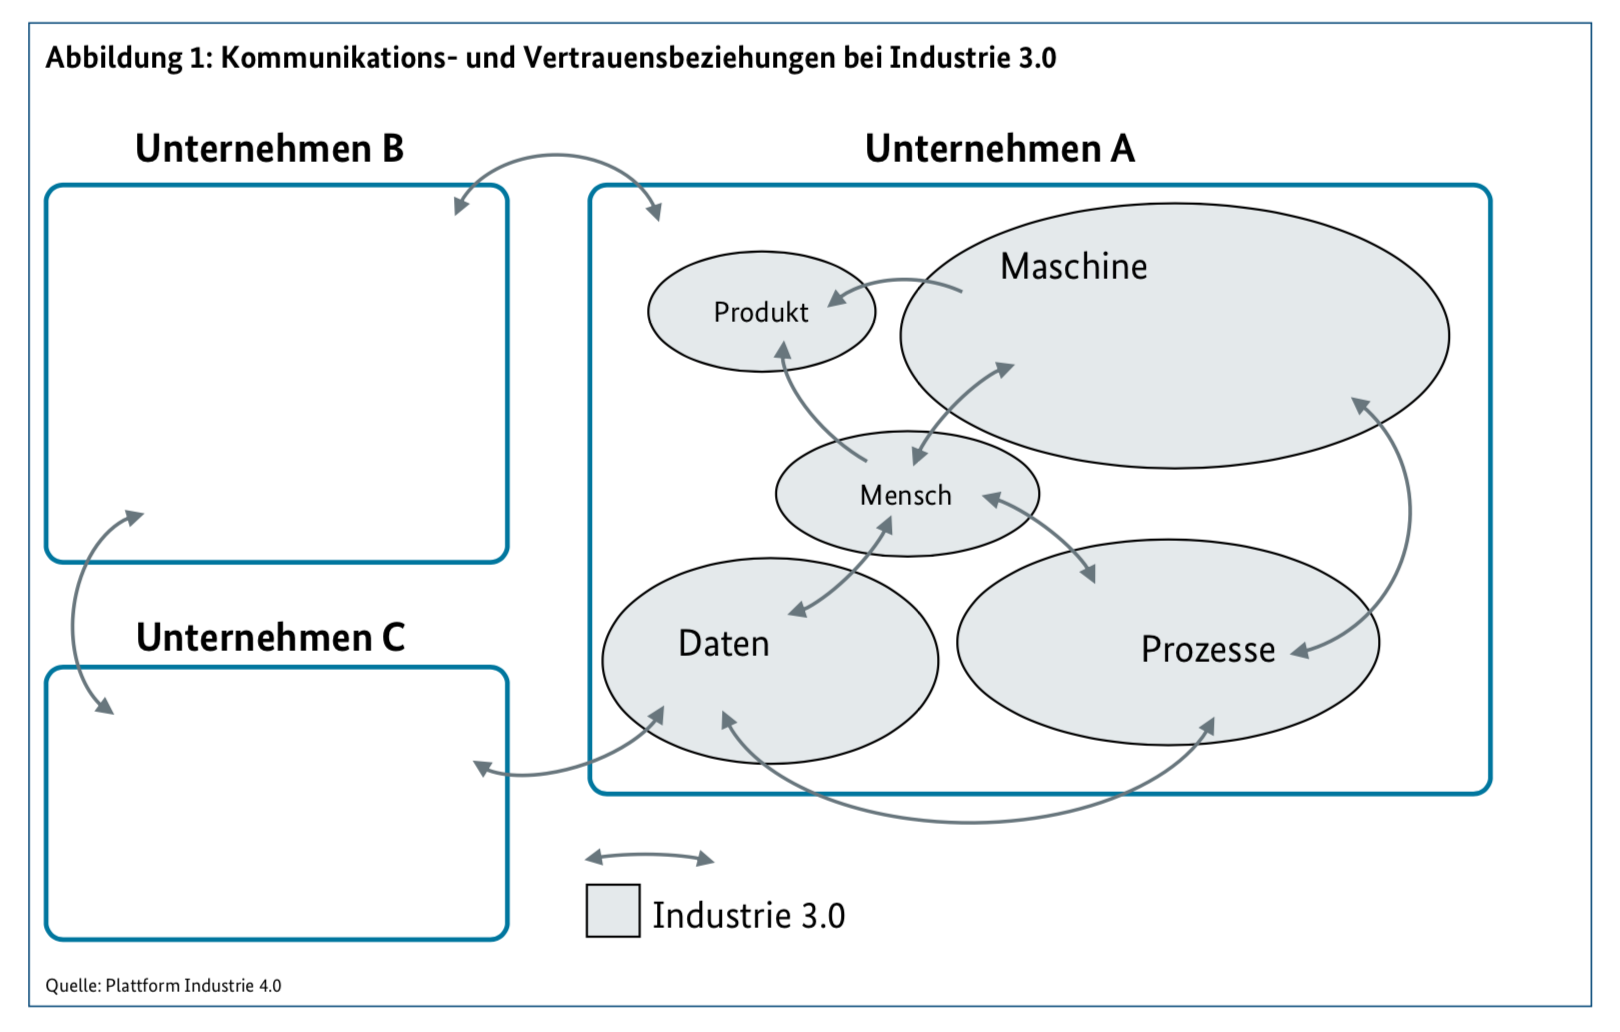
\includegraphics[width=15cm]{kommunikationsbeziehungen-i30}
  \caption{Kommunikationsbeziehungen in einer Industrie 3.0 Umgebung - TODO ref. sichere unternehmensübergreifende Kommunikation}
  \label{Kap2:Industrie3.0-Kommunikation}
\end{figure}

\clearpage

\subsection{4. industrielle Revolution}
Das Ende des 20. Jahrhunderts gilt als der Beginn der 4. industriellen Revolution. Das Kennzeichen dieser Phase ist die zunehmende Digitalisierung. Mit ihr geht die technische Vernetzung physischer Gegenstände, dem \ac{IoT}, einher. Mehr und mehr Geräte oder Gegenstände besitzen die Möglichkeit aktiv durch Datenaustausch oder passiv z. B. mit Hilfe eines Bar- oder QR-Codes mit der digitalen Welt zu kommunizieren und somit eine fortschreitende Automatisierung sowie Individualisierung zu ermöglichen. 

Im Gegensatz zur Industrie 3.0 sollen Maschinen autonom, auch über Unternehmensgrenzen hinweg, miteinander kommunizieren können um gesamte Geschäftsprozesse zu übernehmen. Dies setzt eine Öffnung der Unternehmen nach außen voraus.

\begin{figure}[h]
  \centering
  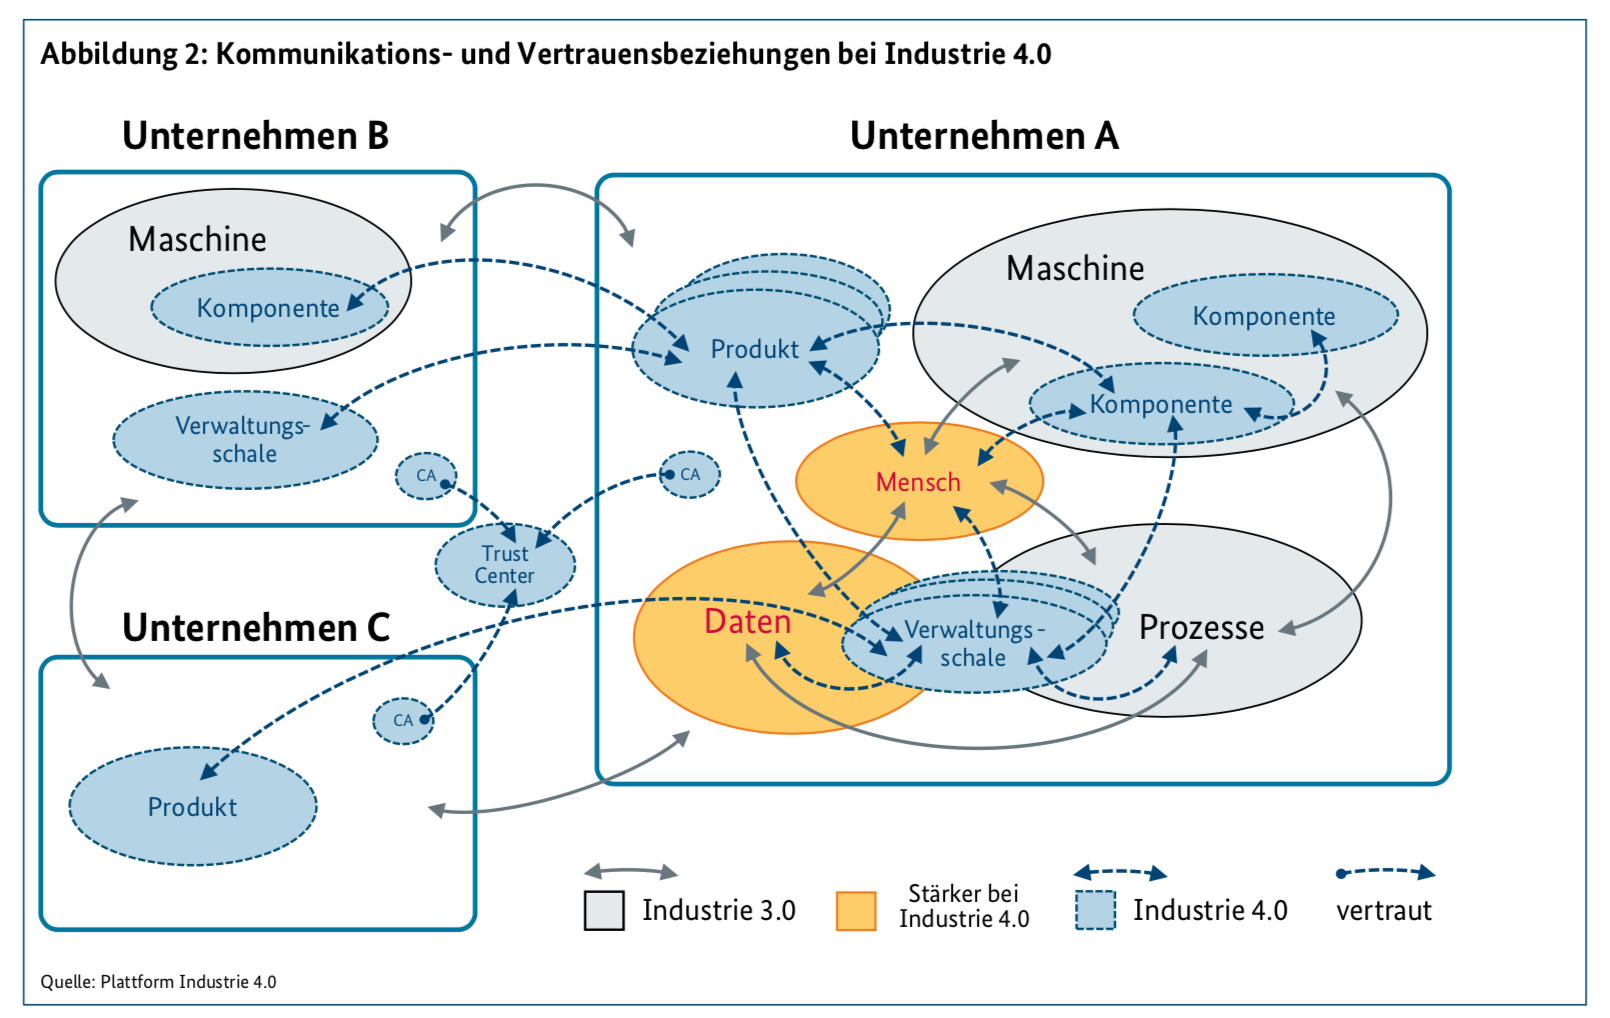
\includegraphics[width=15cm]{kommunikationsbeziehungen-i40}
  \caption{Kommunikationsbeziehungen in einer Industrie 4.0 Umgebung - TODO ref. sichere Unternehmensübergreifende Kommunikation}
  \label{Kap2:Industrie4.0-Kommunikation}
\end{figure}

\clearpage

Diese Entwicklung erzeugt durch die ständige Kommunikation eine große Menge an Daten, welche den Anforderungen der IT-Sicherheit gerecht werden müssen, um Verbraucher und Unternehmen zu schützen.

TODO - bis hierhin auf einen Absatz kürzen -> uninteressant!

\section{aktueller Stand der Technik}
Der Prozess der vierten industriellen Revolution ist ein stetiger, nicht abgeschlossener Prozess. Aktuell werden die ersten Smart Factories der Industrie errichtet und erste smarte Einkaufsmöglichkeiten, wie Amazon Go und TODO - siehe Trumpf, für den Endverbraucher geschaffen. Diese Fabriken und Filialen stellen die ersten ihrer Art dar und dienen als Prototypen. Das Ziel des Wandels in der Strukturierung und Organisation der Produktion in Unternehmen ist eine immer weitere Automatisierung der Prozessabwicklung bis hin zu autonom arbeitenden Fabriken. Für kritische Infrastrukturen, wie z. B. im Energie-, Wasser-, Transport- und Gesundheitssektor existiert diese Verbindung bereits.

Die Umsetzung dieser Innovationen basiert hauptsächlich auf dem Fortschritt der \ac{IT} und dem Einzug der Internet-Technologien in die Industrie. Diese Entwicklung macht es möglich immer schneller Informationen auszutauschen, größere Datenmengen zu analysieren und diese zu verarbeiten. In der Industrie entstehen dadurch u. a. die folgenden Chancen:

\begin{itemize}
  \item Die Kommunikationsinfrastruktur wird in Zukunft in Produktionssystemen so preiswert sein, dass sie sinnvoll für Konfiguration, Service, Diagnose, Bedienung und Wartung genutzt werden kann.
  \item Die Produktionssysteme werden mehr und mehr mit einem Netz verbunden, erhalten dort eine digitale Identität, werden somit such- und analysierbar und besitzen die Möglichkeit Daten über sich selbst zu veröffentlichen. 
  \item Maschinen und Anlagen speichern ihre Zustände in ihrer digitalen Identität im Netz. Diese Zustände sind aktuell, aktualisierbar und zunehmend vollständig. Sind im Netzwerk viele solcher Identitäten vorhanden, können die Daten effizient abgerufen und ausgetauscht werden.
  \item Softwaredienste werden über das Netz verknüpft werden und können somit automatisiert individuelle Aufgaben durch die direkte Kommunikation der Systeme erledigen. Eine solche individuelle Wertschöpfung war bisher nur unwirtschaftlich oder gar nicht möglich.
\end{itemize}

Diese Veränderungen im Wertschöpfungsprozess und die ständige Kommunikation der Systeme bereiten jedoch auch Probleme. Es entstehen große Mengen an Daten, welche u. a. über einen unsicheren Kanal verbreitet werden sollen. Des weiteren sind viele vorhandene Produktionsanlagen nicht für diese Form von vermaschter Kommunikation entwickelt worden. Diesen Problemen wird aktuell durch die Entwicklung von Industriestandards und \ac{M2M}-Protokollen, wie z. B. die \ac{OPC UA} entgegengewirkt. Um vorhandene Anlagen weiterhin nutzen zu können, werden Gateways genutzt. (TODO Trumpf ref.)

\section{Automatisierungspyramide}
\label{Grundlagen:Automatisierungspyramide}
Die Automatisierungspyramide stellt die beteiligten Systeme und Softwarekomponenten eines automatisierten Prozesses systematisch dar. Diese beginnen, ausgehend vom Kundenauftrag und der betriebswirtschaftlichen Planung der Produktion auf der Unternehmensebene im \ac{ERP} System. Die Ergebnisse der Planung werden an das \ac{MES} übergeben, welches die verschiedenen Fertigungs- oder Logistikaufträge generiert. Die Aufträge werden anschließend auf der Prozessleit- (\ac{SCADA}), Steuerungs- (\ac{SPS}) und Feldebene (Ein-/Ausgangssignale) bearbeitet.

\begin{figure}[h]
  \centering
  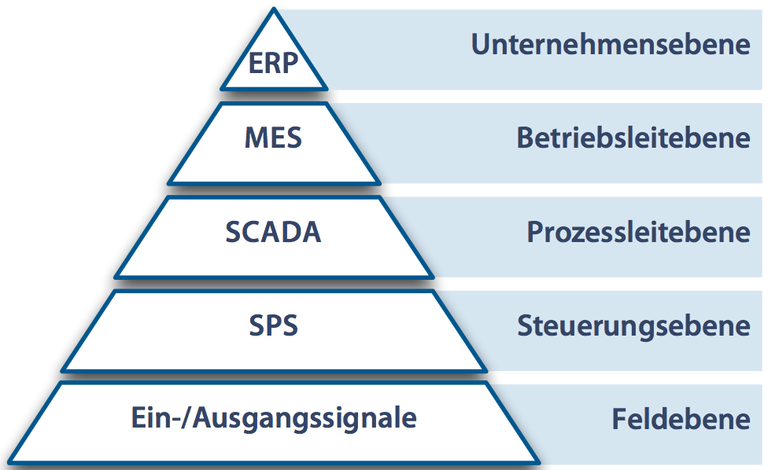
\includegraphics[width=10cm]{automatisierungspyramide}
  \caption{Automatisierungspyramide - TODO ref. Langmann,2004}
  \label{Kap2:Automatisierungspyramide}
\end{figure}

\clearpage

Während die oberen Schichten der Pyramide (\ac{ERP} und \ac{MES}) durch Standardkomponenten bzw. -software der IT realisiert werden, zählen die unteren Schichten (Prozessleit- bis Feldebene) zur Automatisierung, welche die Steuerung und Kontrolle der technischen Anlagen übernimmt. Diese werden auch als Shop-Floor-Ebene bezeichnet. Sie sind durch spezielle Hard- und Softwarelösungen umgesetzt. Die Kommunikation dieser Systeme ist u. a. für spezielle Anwendungsfälle wie harte Echtzeitkommunikation mit Verzögerungen <1ms ausgelegt. Die Integration von Sicherheitsmaßnahmen bei der Kommunikation dieser Systeme stellt oft eine große Herausforderung dar.

\section{Industrie 4.0}
Der Begriff Industrie 4.0 wurde erstmals auf der Hannover Messe 2011 verwendet (\cite{drath2014}) und soll das Ergebnis der 4. industriellen Revolution darstellen. Der Grundgedanke hinter Industrie 4.0 ist die flächendeckende Vernetzung von Informations- und Kommunikationstechnik zu einem Internet der Dinge, Dienste und Daten (\cite{Spath2013}). Diese Vernetzung soll einen ständigen Informationsaustausch zwischen den Komponenten ermöglichen. Jede Komponente des \ac{IoT} soll als \ac{CPS} arbeiten. Ein \ac{CPS} besitzt neben seiner realen Identität eine digitale Identität, über welche es ständig mit anderen \ac{IoT}-Geräten kommunizieren kann. Kunden- und Maschinendaten werden miteinander vernetzt \cite{rami2016}.

\begin{figure}[h]
  \centering
  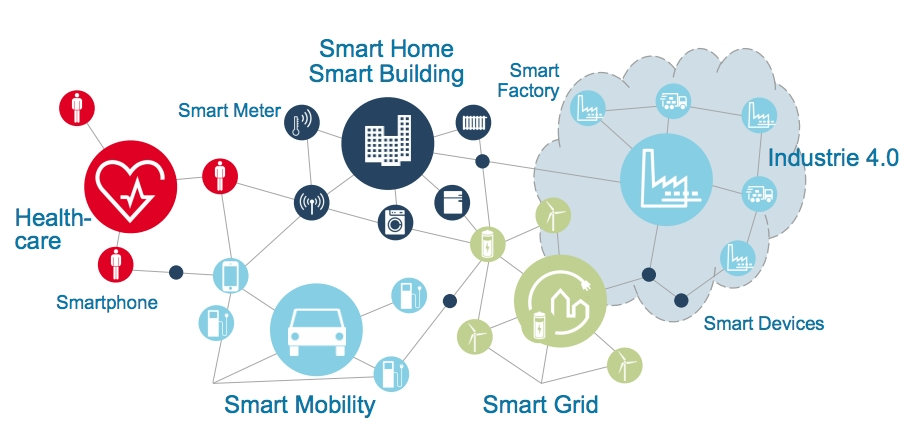
\includegraphics[width=15cm]{internet-der-dinge}
  \caption{Das Internet der Dinge - \cite{rami2016}}
  \label{Kap2:Das Internet der Dinge}
\end{figure}

\clearpage

Für Unternehmen bedeutet dies einen Wechsel von einer linearen Prozesskette hin zu einem vermaschten Netzwerk, in dem jede Komponente mit dem gesamten Netzwerk kommunizieren kann. Dies beinhaltet die Vernetzung der Komponenten auf horizontaler und vertikaler Ebene. Die vertikale Ebene stellt die technischen Komponenten dar und wird durch die Automatisierungspyramide beschrieben. Die horizontale Ebene beschreibt die wirtschaftlichen Geschäfts- bzw. Produktionsprozesse und besteht u. a. aus: Einkauf, Lieferanten, Produktionsplanung, Logistik, Sequenzierung und Lagerverwaltung. Das Ziel ist die Vernetzung aller Beteiligten.

\begin{figure}[h]
  \centering
  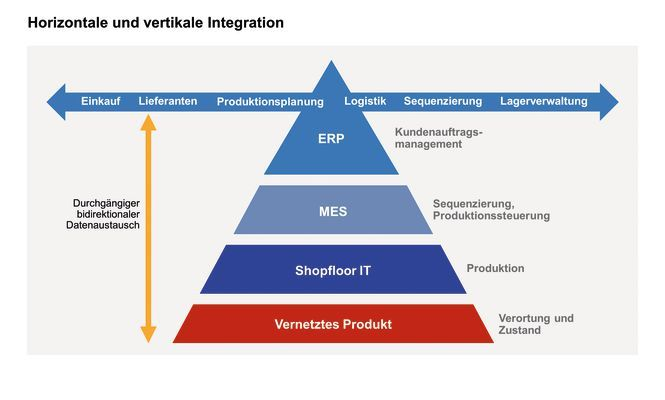
\includegraphics[width=15cm]{horizontalevertikaleIntegration}
  \caption{horizontale und vertikale Integration - TODO ref. HP Industry-of-things siehe bookmark}
  \label{Kap2:horizontale und vertikale Integration}
\end{figure}

\clearpage

\subsection{\ac{IoT}/\ac{IIoT}}
\ac{IoT} beschreibt ein verbraucherorientiertes Konzept für die Nutzung von digitalisierten und vernetzten Systemen. Hierbei werden die physischen Systeme virtuell abgebildet. Dies wird genutzt, um die Effektivität der Systeme zu verbessern und intelligente Services zu nutzen. Das \ac{IIoT} beschreibt den Gebrauch von \ac{IoT}-Technologien im industriellen Raum.

Das \ac{IoT} ist ein wesentlicher Bestandteil der Industrie 4.0, welche Netzwerke aus Systemen, Daten und Dienstleistungen herstellt, in denen diese Komponenten miteinander kommunizieren. Für die Kommunikation haben sich, je nach Anforderungen, verschiedene Protokolle, wie z.B. \ac{HTTP}, \ac{CoAP}, \ac{XMPP} und \ac{MQTT}, etabliert. Jedes dieser Protokolle besitzt für spezifische Anforderungen wie Skalierbarkeit, vorhandene Ressourcen, Echtzeitkommunikation oder Sicherheit Vor- und Nachteile. 

\subsection{Industrial Ethernet}
TODO - Ethernet für Industrieanlagen

\section{Grundprinzipien der sicheren Kommunikation}
\label{Grundlagen:Grundprinzipien der sicheren Kommunikation}
Die Grundprinzipien der sicheren Kommunikation beschreiben die Schutzziele im Bereich der Informationssicherheit. Diese verdeutlichen den Anspruch an die Sicherheit an ein zu implementierendes System oder ein Netzwerk. Sie stellen einen vereinbarten Umfang gegen Bedrohungen dar, welcher von den Kommunikationspartnern gewährleistet wird und nachgewiesen werden kann. Diese klassischen Schutzziele sind auch für Industrie 4.0 Umgebungen zutreffend. Die weitreichende Vernetzung der Systeme in der Industrie 4.0 erfordert jedoch weitere Schutzziele, um einen rechtskonformen Umgang oder besondere Anforderungen sicherzustellen.

\subsection{klassische Schutzziele}
TODO - Hierunter fallen die Bereiche Netzsicherheit und Datensicherheit, Sichere Identitäten und funktionale Sicherheit. Netzsicherheit und Datensicherheit werden in der AG3 der Plattform Industrie 4.0 adressiert. Die UAG Netzkommunikation arbeitet bzgl. dieser Punkte mit der AG3 zusammen. Zum Thema „Security und funktionale Sicherheit“ arbeitet die AG3 mit dem DKE-TBINK AK IT Security und Security by Design zusammen. Hinsichtlich funktionaler Sicherheit gibt es Anforderungen von Seiten IEC 61784-3. Diese müssen bei der Definition neuer Systeme berücksichtigt werden. - TODO

\begin{itemize}
  \item Vertraulichkeit/Zugriffsschutz
  \item (Daten)-Integrität/Änderungsschutz
  \item Authentizität/Fälschungsschutz
  \item Verfügbarkeit
\end{itemize}

\subsection{weitere Schutzziele}
\begin{itemize}
  \item Verbindlichkeit/Nichtabstreitbarkeit: TODO - z.B. rechtliche Anforderungen
  \item Anonymität
\end{itemize}

\section{Anforderungen an Industrie 4.0 Umgebungen}
Aufgrund der unterschiedlichen Einsatzbereiche von Industrie 4.0 Systemen, unterscheiden sich auch dementsprechend deren Anforderungen. Zusätzlich zu den in \autoref{Grundlagen:Grundprinzipien der sicheren Kommunikation} Grundprinzipien der sicheren Kommunikation beschreiben die Referenzmodelle \ac{RAMI4.0} und \ac{IIRA} grundsätzlich drei Anforderungen an den Übertragungskanal \cite{BMWiNeCon2016}.

\subsection{Sicherheit}
\begin{itemize}
    \item Netzsicherheit und Datensicherheit
    \item Sichere Identitäten
    \item funktionale Sicherheit
\end{itemize}

\subsection{Verfügbarkeit}
Die ständige Verfügbarkeit von Daten und Diensten spielt in der Industrie 4.0 eine bedeutende Rolle, um den Datenaustausch zwischen zwei Kommunikationspartnern im Netz jederzeit zu ermöglichen. Als Verfügbarkeit wird die Wahrscheinlichkeit bezeichnet, dass ein System innerhalb eines bestimmten Zeitraumes erreichbar ist. Ein System gilt als verfügbar, wenn es erreichbar ist und die für es vorgesehenen Aufgaben erledigen kann.

Die Verfügbarkeit eines Systems wird in Verfügbarkeitsklassen gegliedert. Diese beschreiben Verfügbarkeitswahrscheinlichkeiten von 99\% ( Verfügbarkeitsklasse 2 ) bis 99,9999\% ( Verfügbarkeitsklasse 6 ). Eine exakte Definition, wann ein System hochverfügbar ist, gibt es nicht - TODO ref. Im Allgemeinen wird ab Verfügbarkeitsklasse 3 ( 99,99\% ) von Hochverfügbarkeit gesprochen.

TODO - Verfügbarkeit gewährleisten durch...

\section{Security by Design}
In der Vergangenheit wurden Sicherheitsmechanismen üblicherweise nachträglich und reaktiv in die Entwicklung von Komponenten mit einbezogen. Industrie 4.0 Umgebungen erfordern umfassende Maßnahmen, um die in \autoref{Grundlagen:Grundprinzipien der sicheren Kommunikation} beschriebenen Schutzziele zu erfüllen und eine sichere Kommunikation zu gewährleisten. Dies gilt vor allem für Maschinenbau- und Fertigungsunternehmen, welche häufig proprietäre Individualsoftware zur Steuerung der Maschinen einsetzen \cite{DTAG2016}. Aus der Notwendigkeit, Sicherheitsaspekte bereits in die Softwareentwicklung mit einzubeziehen und einen Schutz der Kommunikation zu gewährleisten, hat sich der Begriff Security by Design entwickelt.

Die Methoden und Ziele der Angreifer stehen jedoch auch unter einem ständigen Wandel. Somit ist es nicht möglich, eine Securityimplementierung zu entwickeln und diese wiederholt einzusetzen. Vielmehr ist es notwendig, die Sicherheit durch Security by Design so weit als möglich proaktiv herzustellen und gleichzeitig im Schadensfall flexibel und rasch zu reagieren, um das Schadensausmaß zu begrenzen. Es sind Maßnahmen zur Prävention, Detektion und Reaktion erforderlich. TODO - ref. Umsetzungsstrategie Industrie 4.0

\section{Kommunikationsstrukturen in Industrie 4.0 Umgebungen}
Um die Kommunikation zwischen verschiedenen Teilnehmern zu ermöglichen, ergeben sich in der Praxis unterschiedliche Strukturen. Jede dieser Strukturen bietet, je nach Anwendungsfall und zu erfüllenden Anforderungen, Vor- und Nachteile.

TODO - mehr -> siehe sichere Kommunikation-i4.0

\subsection{End2End}
Die Komponenten der Industrie 4.0 Umgebung kommunizieren über einen direkten Kanal miteinander. Dies setzt voraus, dass sich beide Teilnehmer in einem Netzwerk befinden, welches die benötigten Dienste wie z. B. \ac{IP} und \ac{DNS} zur Kommunikation bereitstellt. Des weiteren müssen beide Systeme diese Dienste und Protokolle unterstützen.

\subsection{Gateways}
Um existierende Systeme, welche selbst nicht Industrie 4.0 konform kommunizieren oder zu wenig Rechenleistung besitzen, in die Industrie 4.0 Welt zu integrieren, werden Industrie 4.0 Gateways genutzt. Dabei ist jedoch zu beachten, dass die Systeme hinter den Gateways nicht als Industrie 4.0 Komponenten entwickelt wurden und somit auch keine oder nur wenige dieser Eigenschaften besitzen. Des Weiteren ist es möglich, dass die Kommunikation aus Leistungsgründen oder besonderer Anforderungen über optimierte, proprietäre Protokolle stattfindet. Die Gateways müssen auf die Systeme und deren Protokolle individuell konfiguriert werden, um die Funktionalitäten im Industrie 4.0 Netz bereitstellen zu können, und die Kommunikation zu schützen.

\subsection{Publish-Subscribe}
Das Publish-Subscribe Modell bietet die Möglichkeit Informationen an mehrere Teilnehmer zu verteilen. Hierbei melden sich die Empfänger beim Verteiler an und wählen aus, über welche Nachrichtentypen sie informiert werden möchten. Diese Verteildienste nutzen zur besseren Skalierung und Reduzierung der Netzlast häufig Datagramme wie \ac{UDP}. Durch die Nutzung von Datagrammen geht jedoch die Fehlertoleranz verloren. Somit muss entweder dafür gesorgt werden, dass eine sehr zuverlässige Netzwerkinfrastruktur vorhanden ist und hohe Bandbreitenreserven geschaffen werden, um die Dienstgüte (\ac{QoS}) sicherzustellen oder dieses Modell nur für fehlertolerante Kommunikation wie z. B. Audio- und Video-Anwendungen oder Businessprozesse zu nutzen. 

\subsection{Kommunikation mit Netzwerk als Partner}
Zeitkritische Automatisierungsanwendungen verlangen besondere Netzwerkeigenschaften. Sie können auf Latenz oder Jitter angewiesen sein. Um diese Eigenschaften sicherzustellen, ist es sinnvoll in diese Netze eine Industrie 4.0 Schnittstelle zu integrieren. Somit ist es den Teilnehmern möglich, über die Verwaltungsschale sicherzustellen, dass das Netzwerk die erforderlichen Anforderungen bereitstellt. \cite{sichKom2017}

TODO - Bilder -> sichere-kommunikation-i40

\section{Normen und Standards}
\label{Grundlagen:Normen und Standards}
Im Gegensatz zur Industrie 3.0, in welcher Daten auf lokaler Ebene oder zwischen einzelnen internen Unternehmensebenen ausgetauscht wurden, stellt der Datenaustausch und Informationsfluss im vermaschten Industrie 4.0 Netzwerk einen wesentlichen Bestandteil dar. Aktuell gibt es zwei Architekturmodelle zur Umsetzung von Industrie 4.0 Umgebungen. Diese setzen sich aus dem von der Platform Industrie 4.0 entwickelten \ac{RAMI4.0} und der \ac{IIRA} der \ac{IIC} zusammen. Beide Modelle verfolgen verschiedene Integrationsansätze.

Des Weiteren findet die Kommunikation in der Industrie 4.0 nicht mehr über einzelne, vorgegebene Schnittstellen statt, sondern direkt von den Produktionssystemen, also den unteren Ebenen der Automatisierungspyramide. Um dies zu ermöglichen, ist es notwendig, eine einheitliche Kommunikation durch Normen und Standards herzustellen, um eine unternehmensübergreifende Kommunikation dieser Shop-Floor IT zu ermöglichen. 

\subsection{TCP/IP Referenzmodell}
\label{Grundlagen:TCP/IP Referenzmodell}
Unternehmensübergreifende Kommunikation in Industrie 4.0 Umgebungen findet im wesentlichen über IP-Netze statt. Diese basieren auf dem TCP/IP Referenzmodell, welches ein Schichtenmodell ist und die vier Schichten der Internetprotokollfamilie beschreibt. Sie setzen sich aus Application-, Transport-, Internet- und Link-Layer zusammen. Die Schichten des TCP/IP Referenzmodells überlagern sich mit den Schichten des ISO/OSI Referenzmodells. 

\subsubsection{Application Layer}
Die Anwendungsschicht ist für die Übertragung der Nutzdaten zwischen verschiedenen Anwendungen zuständig. Dabei kann es sich um entfernte Anwendungen handeln. Diese sollen sich für den Benutzer verhalten, als würden sie lokal ausgeführt werden.

TODO - Prozess- und Businesslogik

\subsubsection{Transport Layer}
Die Transportschicht sorgt für die Kommunikation zwischen Prozessen. Die Transportschicht nutzt Ports um verschiedene Dienste zu adressieren. Sie beeinflusst, ob es sich um eine zuverlässige Verbindung ( TCP ) oder nicht ( UDP ) handelt.

TODO - End2End Security

\subsubsection{Internet Layer}
Die Internetschicht wird genutzt, um Daten von einem Teilnehmer im Netzwerk zum anderen zu übertragen. Die Endpunkte im Netzwerk werden durch IP Adressen beschrieben.

\subsubsection{Link Layer}
Der Bitübertragungsschicht beschreibt die Topologie des Netzwerks. Sie stellt die physikalische Verbindung der Netzwerkteilnehmer zur Verfügung.

TODO - Bild Internetprotokollfamilie
TODO - Mit Bild nur kurz erklären und referenzieren, Überschriften entfernen.

\subsection{Industrie 4.0 Referenzarchitekturen}
\subsubsection{\ac{RAMI4.0}}
Um eine flächendeckende Vernetzung zu ermöglichen, muss eine einheitliche Kommunikation geschaffen werden. Die \ac{RAMI4.0} ist eine dreidimensionale Darstellung aller Teilnehmer einer Industrie 4.0 Umgebung und stellt ein Modell einer \ac{SOA} dar. Sie soll eine Verwaltungsschale für Teilnehmer bilden, um eine standardisierte Kommunikation und einfache Inbetriebnahme neuer Komponenten ermöglichen. \cite{rami2016} Die Achsen des \ac{RAMI4.0} bestehen aus:

\begin{itemize}
  \item Achse 1 - Die Hierarchie zeigt die Anlagen, Maschinen sowie das Endprodukt, welche miteinander Vernetzt sind. In diesem Netzwerk werden Funktionen bereitgestellt und Daten ausgetauscht.
  \item Achse 2 - Die Architektur beschreibt - TODO
  \item Achse 3 - Der Produktlebenszyklus wird im Gegensatz zur Industrie 3.0 in das Netzwerk mit eingebunden. Der gesamte Prozess der Produktion, Wartung bis hin zur Verschrottung soll digital erfasst werden.
\end{itemize}

\begin{figure}[h]
  \centering
  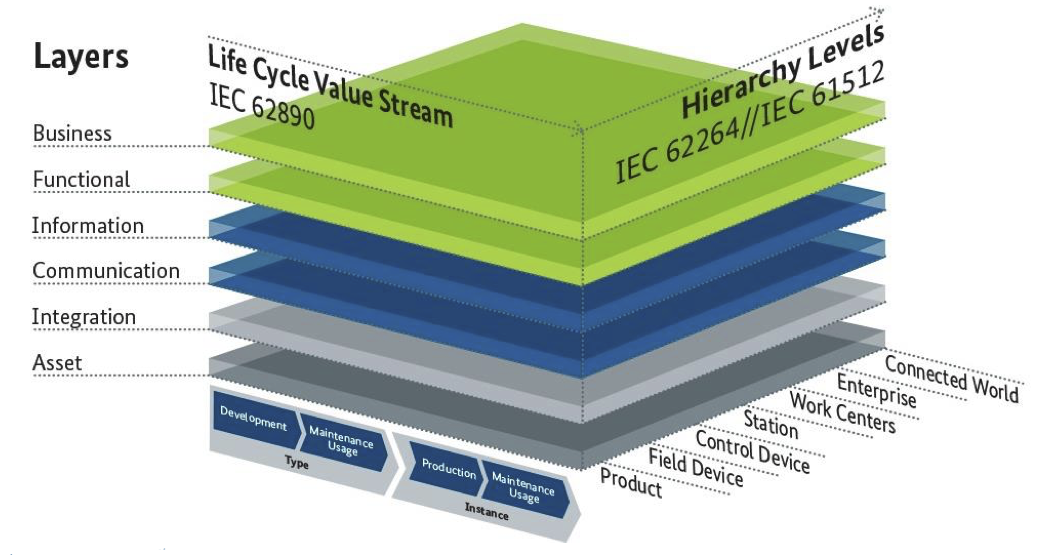
\includegraphics[width=15cm]{rami40}
  \caption{RAMI 4.0 - \cite{rami2016}}
  \label{Kap2:RAMI 4.0}
\end{figure}

\clearpage

Nach dem \ac{RAMI4.0} stellt der Communication Layer das Bindeglied zwischen dem Integration Layer, welcher Eigenschaften der physischen Welt für Computersysteme erreichbar macht, und dem Information Layer, welcher die Funktionsbezogenen Daten beinhaltet, dar. \cite{BMWiNeCon2016} 

TODO - Kommunikation beschreiben - Assets, Verwaltungsschale

Jeder Teilnehmer der Architektur wird als Asset bezeichnet und besitzt seine eigene Verwaltungsschale, welche als Schnittstelle zum Austausch von Informationen dient. Die Verwaltungsschale ist der Übergang zwischen der physischen zur digitalen Welt.

TODO - genauer auf die einzelnen Komponenten eingehen! - Assets, Architektur, Komponenten, Verwaltungsschale
TODO - Architektur wichtig SOA beschreiben -> Angriffsvektoren
TODO - siehe DIN 91345
TODO - Anforderungen an diese Komponenten unterschiedlich

\subsubsection{IIRA}
Das \ac{IIC} veröffentlichte im Jahr 2015 die \ac{IIRA}. Sie beschreibt eine standardbasierte, offene Referenzarchitektur für \ac{IIoT}, welches auf dem \ac{IIAF} basiert. Das \ac{IIAF} unterstützt die Unternehmen bei der Entwicklung, Dokumentation, Kommunikation und Bereitstellung von Systemen im \ac{IIoT} Bereich \cite{iira2017}. Die Beschreibung der Architektur findet mit einem hohen Maß an Abstraktion statt, um das breite Feld der verschiedenen Industrielösungen abdecken zu können und standardisierte Vorgehensweisen bereitzustellen.

TODO - Diese beinhalten niedrige Latenzen und Schwankungen, einen hohen Durchsatz, Skalierbarkeit, Ausfallsicherheit, Datensicherheit und ‚Quality of Service’ (QoS)

\paragraph{Framework}\mbox{}\\
Das \ac{IIAF} folgt der Vorgehensweise des ISO/IEC/IEEE Standard 42010:2011 Systems and Software Engineering–Architecture Description. Concern, Stakeholder und Viewpoint werden als Architecture Frame dargestellt. Die Views und Models als ihre Architecture Representations.

\begin{figure}[h]
  \centering
  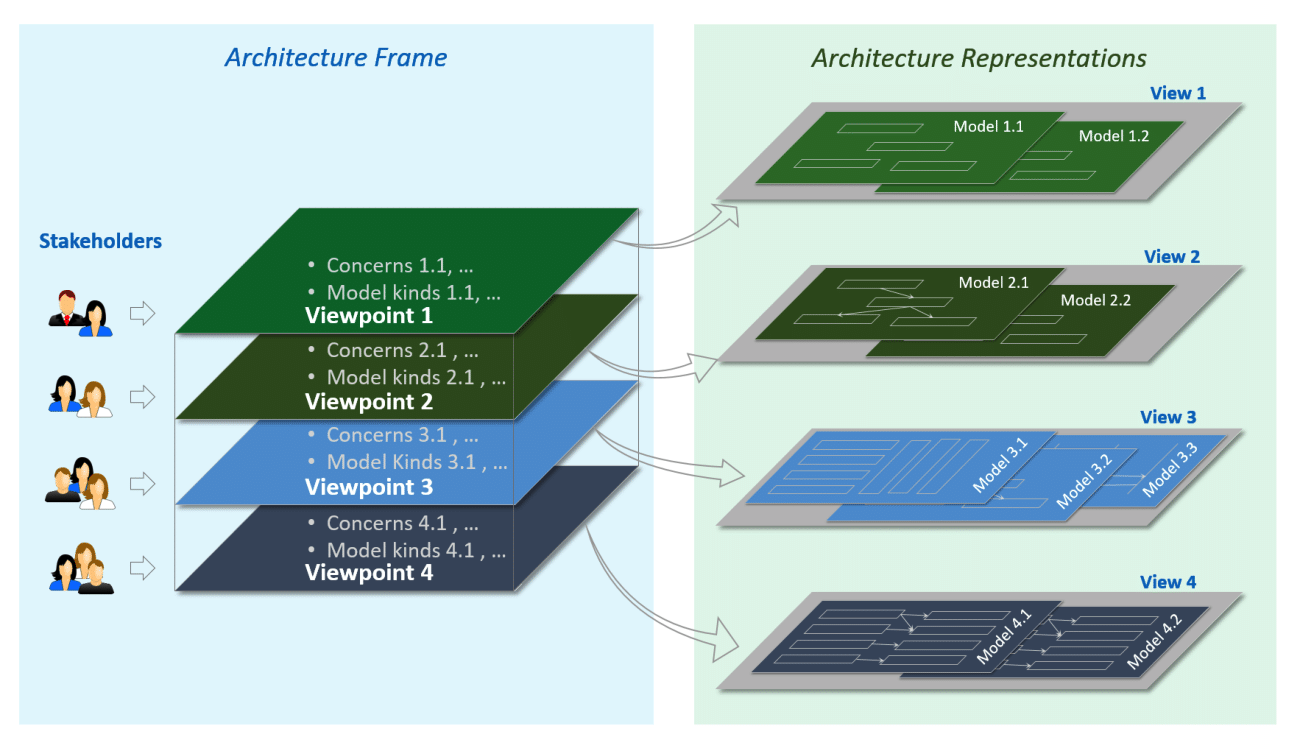
\includegraphics[width=15cm]{iiaf}
  \caption{IIRA - Architekturframework} 
  \label{Kap2:IIRA - Architekturframework}
\end{figure}

\clearpage

\paragraph{Referenzarchitektur}\mbox{}\\
Die \ac{IIRA} ist das Ergebnis der Anwendung des \ac{IIAF} auf die \ac{IIoT} Systeme eines Unternehmens. Sie beschreibt bekannte Risiken beim Betrieb von \ac{IIoT} Systemen in verschiedensten Industriebereichen und Klassifiziert diese mit ihren zugehörigen Stakeholdern in Viewpoints. Anschließend dient die Referenzarchitektur der Beschreibung, Analyse und Behebung dieser Bedenken/Risiken in den einzelnen Viewpoints.

Abbildung \autoref{Kap2:IIAF/IIRA - Übersicht} beschreibt die grundlegende Idee und den Aufbau der \ac{IIRA}.

\begin{figure}[h]
  \centering
  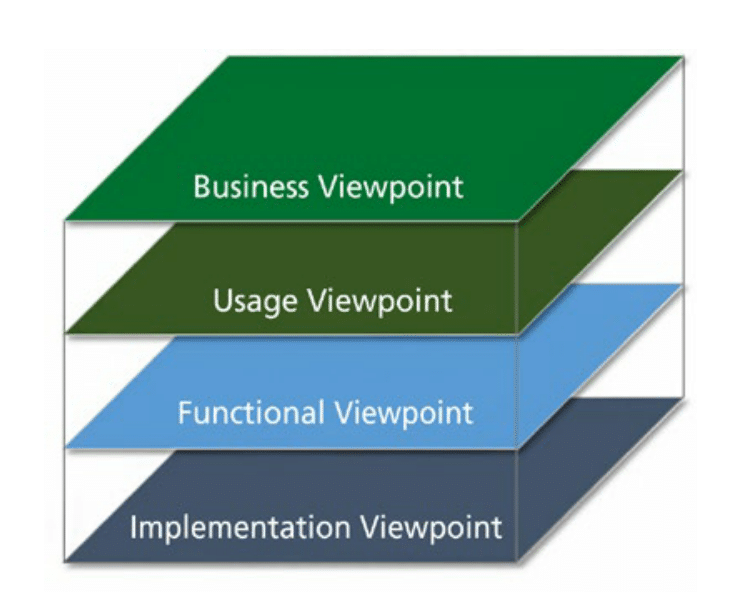
\includegraphics[width=15cm]{iira}
  \caption{IIAF/IIRA - Übersicht} 
  \label{Kap2:IIAF/IIRA - Übersicht}
\end{figure}

\clearpage

\subsection{Protokollstandards}
Durch die vorausgesetzte M2M-Kommunikation wurde die Entwicklung neuer Protokolle zum effizienten Informationsaustausch vorangetrieben, welche es ermöglichen sollen, eine Standardisierung bereitzustellen und somit eine herstellerübergreifende und plattformunabhängige Kommunikation zu ermöglichen. Hierbei haben sich bzgl. der Referenzarchitekturen \ac{RAMI4.0} und \ac{IIRA} die \ac{M2M}-Kommunikationsstandards \ac{OPC UA} und \ac{DDS} etabliert.

\subsubsection{\ac{OPC UA}}
Die \ac{OPC UA} ist ein plattformunabhängiger \ac{IEC} Standard, welcher die \ac{M2M}-Kommunikation zwischen unterschiedlichen Geräten und Systemen der Industrie über verschiedene Netzwerktopologien bereitstellt. Der Standard basiert auf dem Informationsmodell, definiert eine \ac{SOA} und ermöglicht eine robuste und sichere eine Ende zu Ende Kommunikation nach den Vorschriften der TODO ref. - DIN. Er erfüllt die Anforderungen des \ac{RAMI4.0} und etabliert sich zunehmend im Maschinen- und Anlagenbau.

Der Standard wird in 14 geschichteten Spezifikationen beschrieben, welche sich in die Bereiche Core, Access Type und Utility unterteilen lassen. Dabei stellen die Spezifikationen 1-7 sowie 14 die Kernfunktionalitäten des Standards dar. Sie beschreiben die Struktur des OPC Addressraums und der Dienste, die darauf operieren. Die Spezifikationen 8-11 wenden diese Kernfunktionalitäten auf spezifische OPC COM Spezifikationen, wie \ac{DA}, \ac{AE} und \ac{HDA} an. Die Teile 12 und 13 beinhalten Mechanismen zur Discovery von Systemen und beschreiben Möglichkeiten der Datenaggregation.

\begin{figure}[h]
  \centering
  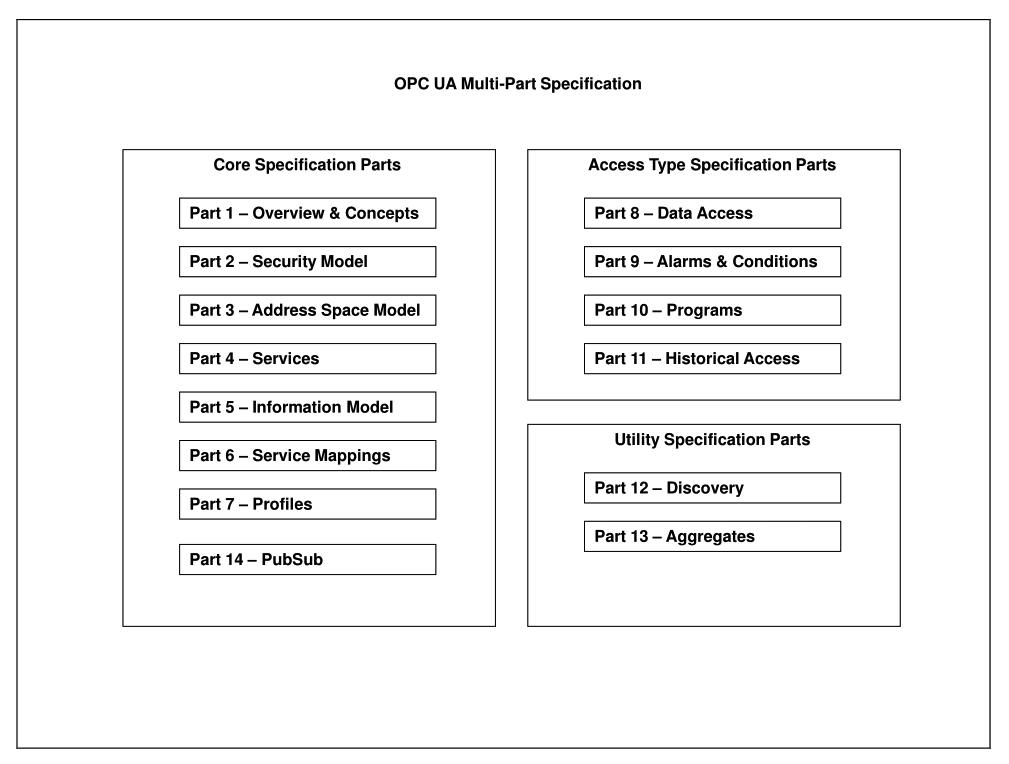
\includegraphics[width=15cm]{opcua-spezifikation}
  \caption{OPC UA Multi-Part Specification - \cite{opcpt1}} 
  \label{Kap2:OPC UA Multi-Part Specification}
\end{figure}

\clearpage

Die \ac{OPC UA} stellt ein Informationsmodell mit Hilfe einer \ac{SOA} bereit. Das Lesen- und Schreiben von Daten in Industrie 4.0 Umgebungen findet durch die Verwaltungsschale der Komponenten statt. Diese wird im \ac{OPC UA} Stack durch den Addressraum beschrieben. Der Adressraum wird zur Speicherung von Knoten, deren Attribute und Referenzen zu anderen Knoten genutzt. Der Addressraum und das Informationsmodell von \ac{OPC UA} werden in den Spezifikationsteilen 3 \cite{opcpc3} und 5 \cite{opcpt5} beschrieben.

Im folgenden Abschnitt wird sich auf die Darstellung der Bestandteile von \ac{OPC UA}, welche an der Netzwerkkommunikation beteiligt sind, beschränkt.

\paragraph{Kommunikationsmodell}\mbox{}\\
\ac{OPC UA} ermöglicht die Kommunikation der Assets über ein Client-Server Pattern. Die Architektur setzt sich dabei aus einem \ac{OPC UA} Client und einem \ac{OPC UA} Server zusammen. Der \ac{OPC UA} Server stellt verschiedene Funktionen bereit, auf welche der \ac{OPC UA} Client mit Hilfe eines Request zugreifen kann. Des Weiteren ist es möglich durch einen Request des \ac{OPC UA} Clients ein Element des Servers beobachten zu lassen, um bei Änderungen vom Server benachrichtigt zu werden. Um die Kommunikation zwischen \ac{OPC UA} Servern zu gewährleisten, ist es möglich einen \ac{OPC UA} Client in einen \ac{OPC UA} Server zu integrieren. In der Grafik \autoref{Kap2:OPC UA Client-Server Architektur} wird das Client-Server Pattern der \ac{OPC UA} Spezifikation schematisch dargestellt. Die linke Seite der Grafik beschreibt die Kommunikation zwischen einem Client und einem Server mit eingebettetem Client. In der rechten Seite der Grafik findet die Kommunikation zwischen dem eingebetteten Client und einem \ac{OPC UA} Server statt.

\begin{figure}[h]
  \centering
  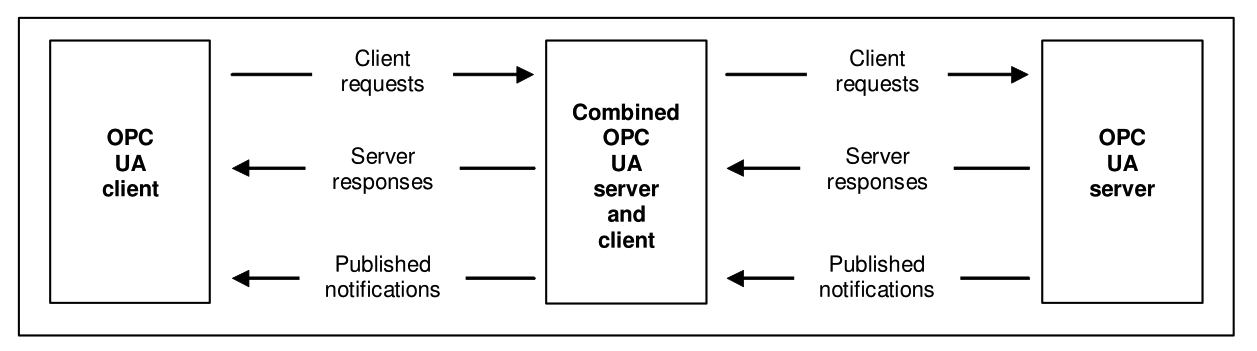
\includegraphics[width=15cm]{opcuaclient-server}
  \caption{OPC UA Client-Server Architektur - \cite{opcpt1}} 
  \label{Kap2:OPC UA Client-Server Architektur}
\end{figure}

Im Jahr 2018 wurde der Standard zusätzlich um eine Spezifikation für das Publish-Subscribe Pattern - TODO ref. - erweitert \cite{hoppe2018}. Das Publish-Subscribe Modell ermöglicht die Nutzung von \ac{OPC UA} in \ac{WAN} Umgebungen durch die Verwendung von Protokollen wie \ac{MQTT} und \ac{AMQP}, während die Ende zu Ende Sicherheit und die standardisierte Datenmodellierung erhalten bleiben. Das Publish-Subscribe Modell ermöglicht die Verwendung des fehlertoleranten Datagramms \ac{UDP}, wodurch geringe Latenzen ermöglicht werden können. 

\paragraph{Kommunikationswege}\mbox{}\\
Die Kommunikation zwischen \ac{OPC UA} Komponenten findet auf der Anwendungsschicht des \ac{TCP}/\ac{IP} Referenzmodells statt und basiert auf dem Protokoll \ac{TCP}/\ac{IP}. Grundsätzlich stellt \ac{OPC UA} die drei Kommunikationswege Binary, Hybrid und Webservice bereit.

\begin{figure}[h]
  \centering
  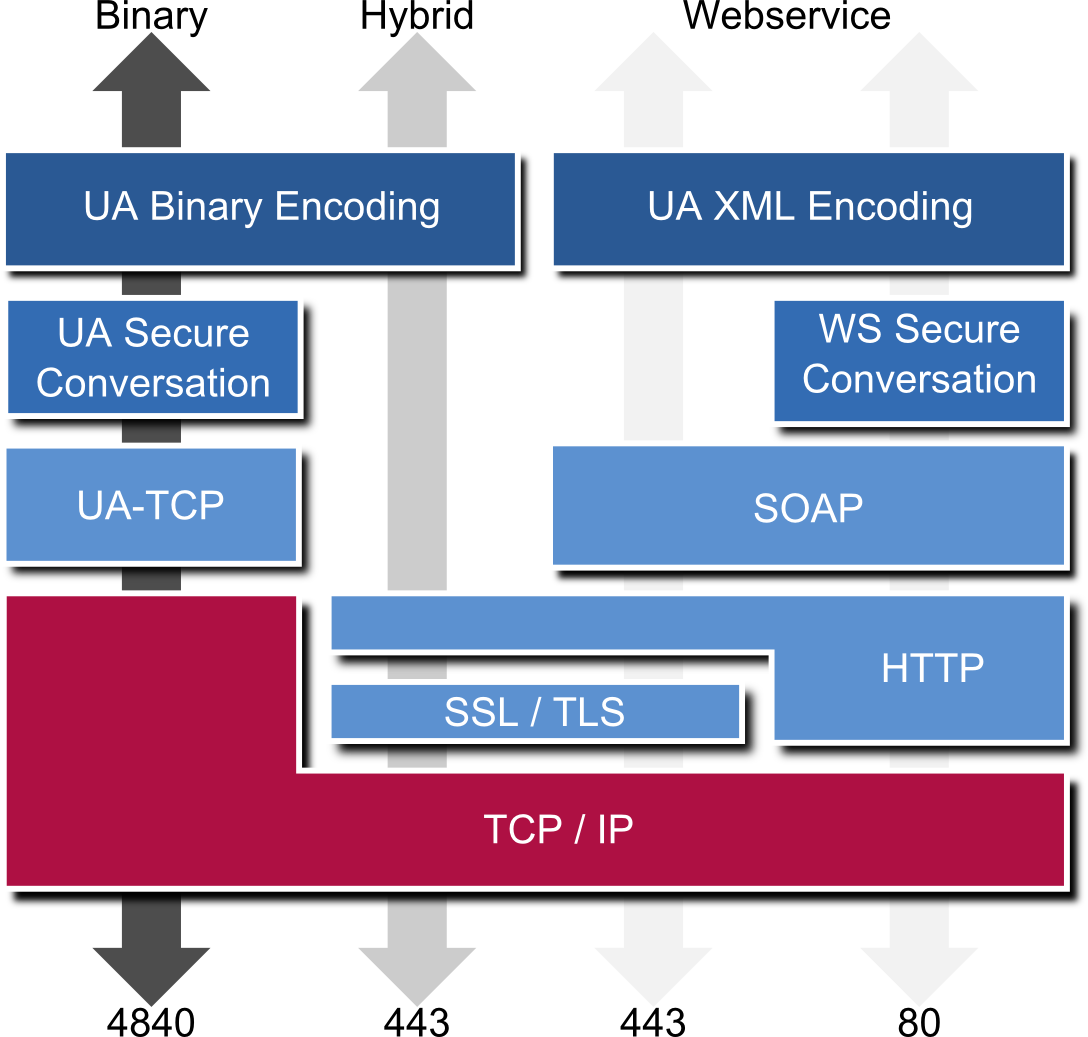
\includegraphics[width=15cm]{opcuaprotocol}
  \caption{OPC UA Kommunikationswege} 
  \label{Kap2:OPC UA Kommunikationswege}
\end{figure}

\clearpage

TODO - Binary
TODO - Hybrid
TODO - Webservice

\paragraph{Sicherheit}
TODO - siehe OPC UA Part 2

\subsubsection{\ac{DDS}}
\ac{DDS} ist ein offener Standard der \ac{OMG} und stellt eine \ac{MOM} zur Kommunikation in hochdynamischen verteilten Systemen dar. Er wurde für niedrige Latenzzeiten, einen hohen Datendurchsatz und eine skalierbare, belastbase und sichere Datenverteilung entwickelt, um die Kommunikation in Steuerungs- und Kontrollaufgaben zu realisieren. Der beschriebene Standard deckt alle Anforderungen der \ac{IIRA} ab und hat sich bereits in industriellen Systemen etabliert. Gegenüber \ac{OPC UA} beschreibt \ac{DDS} eine dezentralisierte Architektur. Es bietet ein Konnektivitäts-Framework, welches ein Kommunikationsparadigma basierend auf einem Shared Data Model, einen Standard für die Definition domain-spezifischer Informationsmodelle, ein starkes Sicherheitsmodell, Discovery und reichhal­tige APIs beinhaltet. Die Kommunikation findet direkt vom Publisher zum Subscriber statt. Dabei werden Latenzzeiten reduziert und durch die Nutzung von Multicast die Netzlast beim Bereitstellen von Informationen an viele Empfänger gering gehalten. Es ist möglich die \ac{MOM} \ac{DDS} in eine \ac{OPC UA} Architektur zu integrieren und mit dem Informationsmodell nutzen.

\section{Testsystem}
\label{Grundlagen:Testsystem}
Die aus der Analyse hervorgehenden möglichen Schwachstellen und Bedrohungen im Bereich der Netzwerksicherheit in Industrie 4.0 Umgebungen und deren Auswirkungen sollen anhand eines vorhandenen, prototypischen Industrie 4.0 Testsystems \cite{Weber2018} veranschaulicht werden. Das vorhandene System setzt die drei Schichten der Software-Architektur (Verteilungs-, Baustein- und Laufzeitschicht) nach Starke / Hruschka um. Die Netzwerkkommunikation wird über das Protokoll \ac{OPC UA} realisiert, welches die Anforderungen der Industrie 4.0 und \ac{RAMI4.0} umsetzt.

\subsection{Architektur}
Das vorhandene System ist, aufgrund der vorgesehenen Einsatzgebiete Lehre, Integrations- und Sicherheitstests, als \ac{VM} umgesetzt worden. Dies ermöglicht es die Testinfrastruktur vom restlichen Netz zu kapseln. Das Betriebssystem der \ac{VM} stellt eine Firewall bereit, welche unerwünschten Netzwerktraffic von oder zu dem System verhindert. Um eine gute Erweiterbarkeit der Testumgebung und Modularisierung der Komponenten zu erreichen, werden die einzelnen Industrie 4.0 Komponenten mit Hilfe der Containerlösung Docker isoliert ausgeführt, verwaltet und deren Netzwerkkommunikation sichergestellt. Durch den zusätzlichen Einsatz des Deploymentsystems Kubernetes wird ein verteiltes Ausführen des Systems ermöglicht und somit eine gute Skalierbarkeit erreicht. 

\subsection{Komponenten}

\subsubsection{Repository}
\subsubsection{Discovery Server}
\subsubsection{\ac{PKI}}
\subsubsection{Identity Provider}
\subsubsection{Verwaltungsinterface}
\subsubsection{Scheduler}